\documentclass[10pt,a4paper]{article}
\usepackage[utf8]{inputenc}
\usepackage[italian]{babel}
\usepackage{amsmath}
\usepackage{amsfonts}
\usepackage{amssymb}
\usepackage{graphicx}
\usepackage[left=2cm,right=2cm,top=2cm,bottom=2cm]{geometry}
\newcommand{\rem}[1]{[\emph{#1}]}

\author{Gruppo AC \\ Federico Belliardo, Giulia Franchi, Francesco Mazzoncini}
\title{Esercitazione N.6: Amplificatore operazionale: circuiti lineari}
\begin{document}
\section{Scopo dell'esperienza}

Misurare le caratteristiche di amplificatori invertenti e non invertenti realizzati con un op-amp TL081 in fig.\ref{pin}.
\begin{figure}[!htb]
  \centering
  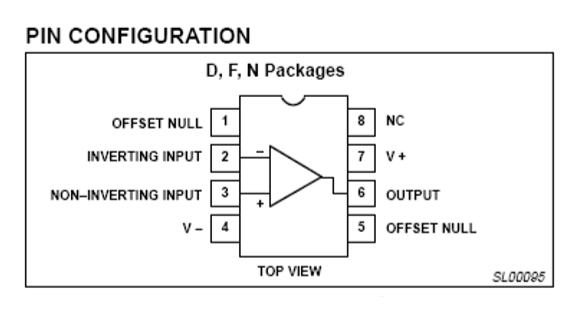
\includegraphics[scale=0.3]{pinrelaz6.png}
\caption{configurazione pin.}
\label{pin}
\end{figure}

\section{Amplificatore invertente}
\subsection{Realizzazione circuito}
Si vuole realizzare un amplificatore invertente con un'impedenza di ingresso superiore a $1k\Omega$ e con un amplificazione di 10. 
Per fare ciò abbiamo montato il circuito in fig. \ref{opampinvert}: Tale circuito infatti presenta una  resistenza di ingresso $R_{in}=R_1$ e un'amplificazione  $A_V=R_2/R_1$ 
Si sono scelte $R_1=$ e $R_2=$ e abbiamo inoltre misurato le  tensioni di alimentazione dell'OpAmp $V_+=$ $V_-=$.
Con questo circuito la resistenza interna attesa è quindi $R_{in.ATT}=$ e $A_{V.ATT}=$ in accordo con le richieste.
\begin{figure}[!htb]
  \centering
  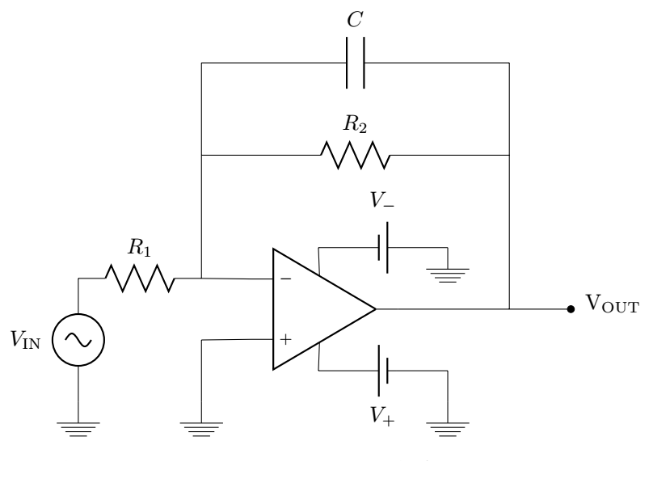
\includegraphics[scale=0.5]{opampinvert.png}
\caption{amplificatore invertente.}
\label{opampinvert}
\end{figure}
\subsection{Misura del guadagno a frequenza fissata}
Abbiamo misurato per un segnale sinusoidale di frequenza $f=$ la tensione picco-picco $V_{OUT}$ in funzione di $V_{IN}$(sempre picco-picco) riportando i dati nella tabella \ref{}. Abbiamo interrotto la presa dati al valore della tensione in ingresso per il quale abbiamo osservato clipping, misurando però anche il massimo valore della tensione in uscita  $V_{OUT} = $ \rem{ controllare con il datasheet}
Abbiamo eseguito inoltre un grafico di $V_{OUT}$ in funzione di $V_{IN}$ e un fit con una retta riportato in fig. \ref{} ricavando come guadagno $A_V=$.

\subsection{Misura dell'impedenza d'ingresso}
Abbiamo misurato la tensione di uscita del circuito a $V_{IN}=$, in modo da evitare fenomeni di clipping, dapprima con lo stesso circuito,poi successivamente aggiugendo una resistenza $R_S=$\footnote{$R_S$ è stata scelta dello stesso ordine della resistenza interna attesa,in modo da non alterare troppo il circuito, ma più grande, in modo da minimizzare l'incertezza} in serie al generatore di funzioni, ottenendo rispettivamente $V_1=$ e $V_2=$ Dalla formula del partitore otteniamo $R_S/R_{IN}=V1/V2-1=$
\section{Risposta in frequenza del circuito e slew rate}
\subsection{Misura della risposta in frequenza}
Abbiamo studiato la risposta in frequenza del circuito misurando $V_{OUT}$ al variare della frequenza (scegliere l'intervallo) con $V_{IN}=$  sinusoidale fissata \footnote{$V_{IN}$ è stata scelta in modo da non avere effetti di distorsione e ci siamo accertati che non variasse al variare della frequenza}.
I dati ottenuto sono stati riportati nella tabella \ref{} e sono stati graficati in un diagramma di Bode
Abbiamo notato che il circuito si comporta come un filtro passa-basso ed abbiamo quindi  eseguito un fit con la funzione $ A=\frac{A_{MAX}}{\sqrt{1+(f/f_t)^2}}$
\rem{vedere se Amax è compatibile con il guadagno massimo dei primi punti}


\subsection{Slew rate}
Abbiamo impostato il generatore di funzioni in modo che fornisse al circuito un’onda quadra di ampiezza $V_{IN} =$ e frequenza $f=$. abbiamo in seguito studiato l'andamento di $V_{OUT}$ nella parte del segnale corrispondente al transiente fra i due stati dell’onda:la tensione osservata presenta inizialmente un andamento qualitativamente esponenziale,successivamente un andamento lineare per poi rallentare in prossimità del suo valore limite. Nella zona di crescita lineare si è dunque presa una misura della differenza di tensione$dV_{OUT}$= relativa a un piccolo intervallo di tempo $dt=$.. Dal loro rapporto si ottiene il valore dello $\emph{slew rate}=$.
\rem{da confrontare con il valore dato dal costruttore}
\section{Amplificatore non invertente}
Abbiamo montato il circuito in fig. \ref{opampnoninvert} con $R_1=$ e  un potenziometro di resistenza massima $P_{1_{MAX}}=$.
\begin{figure}[!htb]
  \centering
  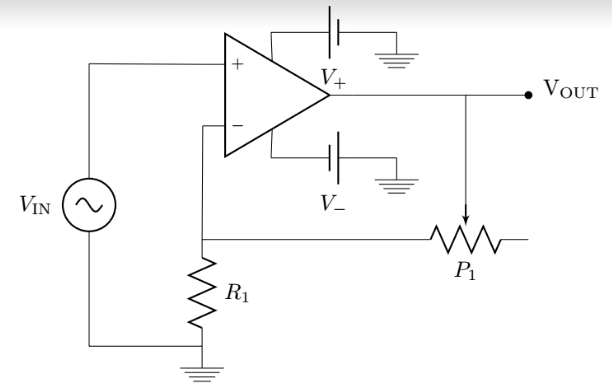
\includegraphics[scale=0.5]{opampnoninvert.png}
\caption{amplificatore non invertente.}
\label{opampnoninvert}
\end{figure}

abbiamo utilizzato come segnale di ingresso fornito dal generatore di funzioni  un onda sinusoidale di ampiezza $V_{IN}=$ \footnote{Anche in questo caso  ci siamo accertati che l'ampiezza del segnale in ingresso rimanesse costante al variare della frequenza, avendo cura in caso di necessità di agire sul generatore di funzioni in modo da avere il segnale voluto} 
\end{document}